\chapter{Analisis}

\section{Template}
Website BlueTape terdiri dari beberapa template yang disimpan di path BlueTape/www/application/views/template yaitu:
\begin{enumerate}
	\item \verb|flashmessage.php| : Template berisi kode php yang akan memberi tahu user apabila proses yang dilakukan terjadi error atau memiliki informasi tertentu.
	\item \verb|head_loggedin.php| : Bagian \texttt{<head>} yang medefinisikan seluruh file css beserta plugin yang digunakan.
	\item \verb|script_foundation| : Bagian yang mendefinisikan seluruh file javascript yang digunakan oleh framework.
	\item \verb|topbar_loggedin.php| : Template berisi navigation bar yang terdiri menu - menu.
\end{itemize}


\section{Antarmuka Cetak Transkrip}
Isi dari halaman antarmuka cetak transkrip terdiri dari dua bagian yaitu :
\begin{enumerate}
	\item \verb|Permohonan Baru| : Sistem akan memberikan dua tampilan untuk bagian ini, dengan kondisi sebagai berikut:
	\begin{itemize}
		\item Sistem akan menampilkan form pengajuan transkrip, apabila mahasiswa belum pernah mengajukan permohonan atau pengajuan sebelumnya  dikonfirmasi staf TU, maka mahasiswa dapat mengajukan permohonan baru.
		\item Sistem akan menampilkan informasi "Anda tidak bisa meminta cetak karena ada permintaan lain yang belum selesai", apabila mahasiswa memiliki pengajuan permohonan transkrip yang belum dikonfirmasi staf TU. 
	\end{itemize}
	\item \verb|Histori Permohonan| : Tabel untuk menampilkan informasi permohonan transkrip seorang mahasiswa. Status, tanggal pembuatan, tipe transkrip, tanggal cetak keterangan dan aksi. 
\end{enumerate}
\begin{figure} [H]
	\centering  
	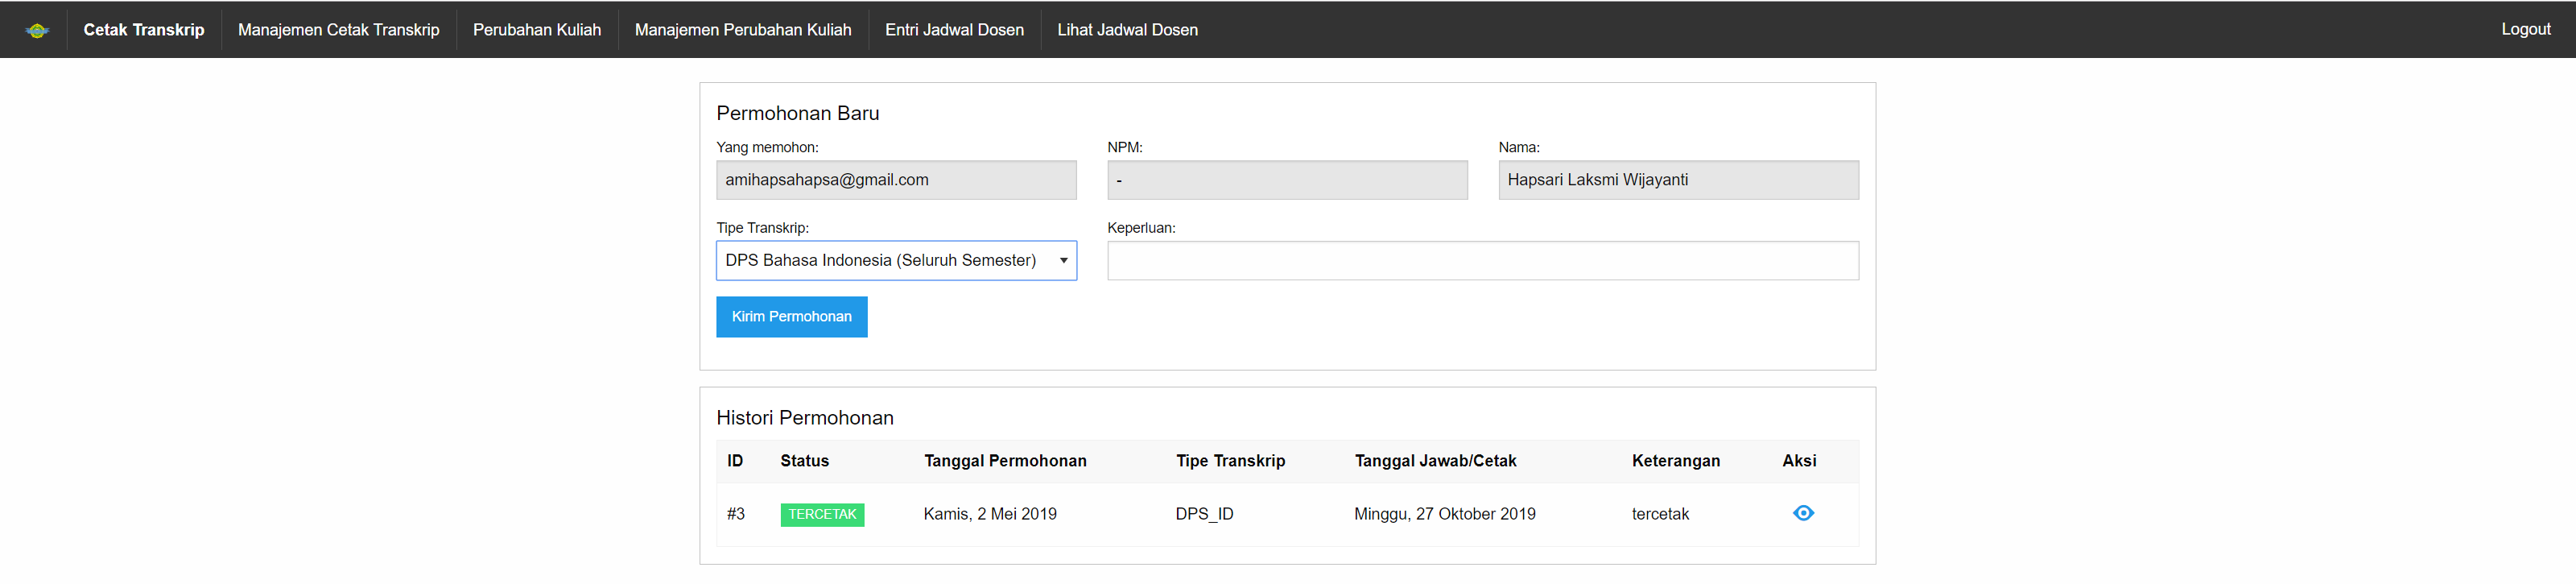
\includegraphics[scale=0.5]{Tampilan-Mahasiswa-Cetak-Transkrip.png}  
	\caption{Antarmuka Cetak Transkrip bagian 1} 
\end{figure}
\begin{figure} [H]
	\centering  
	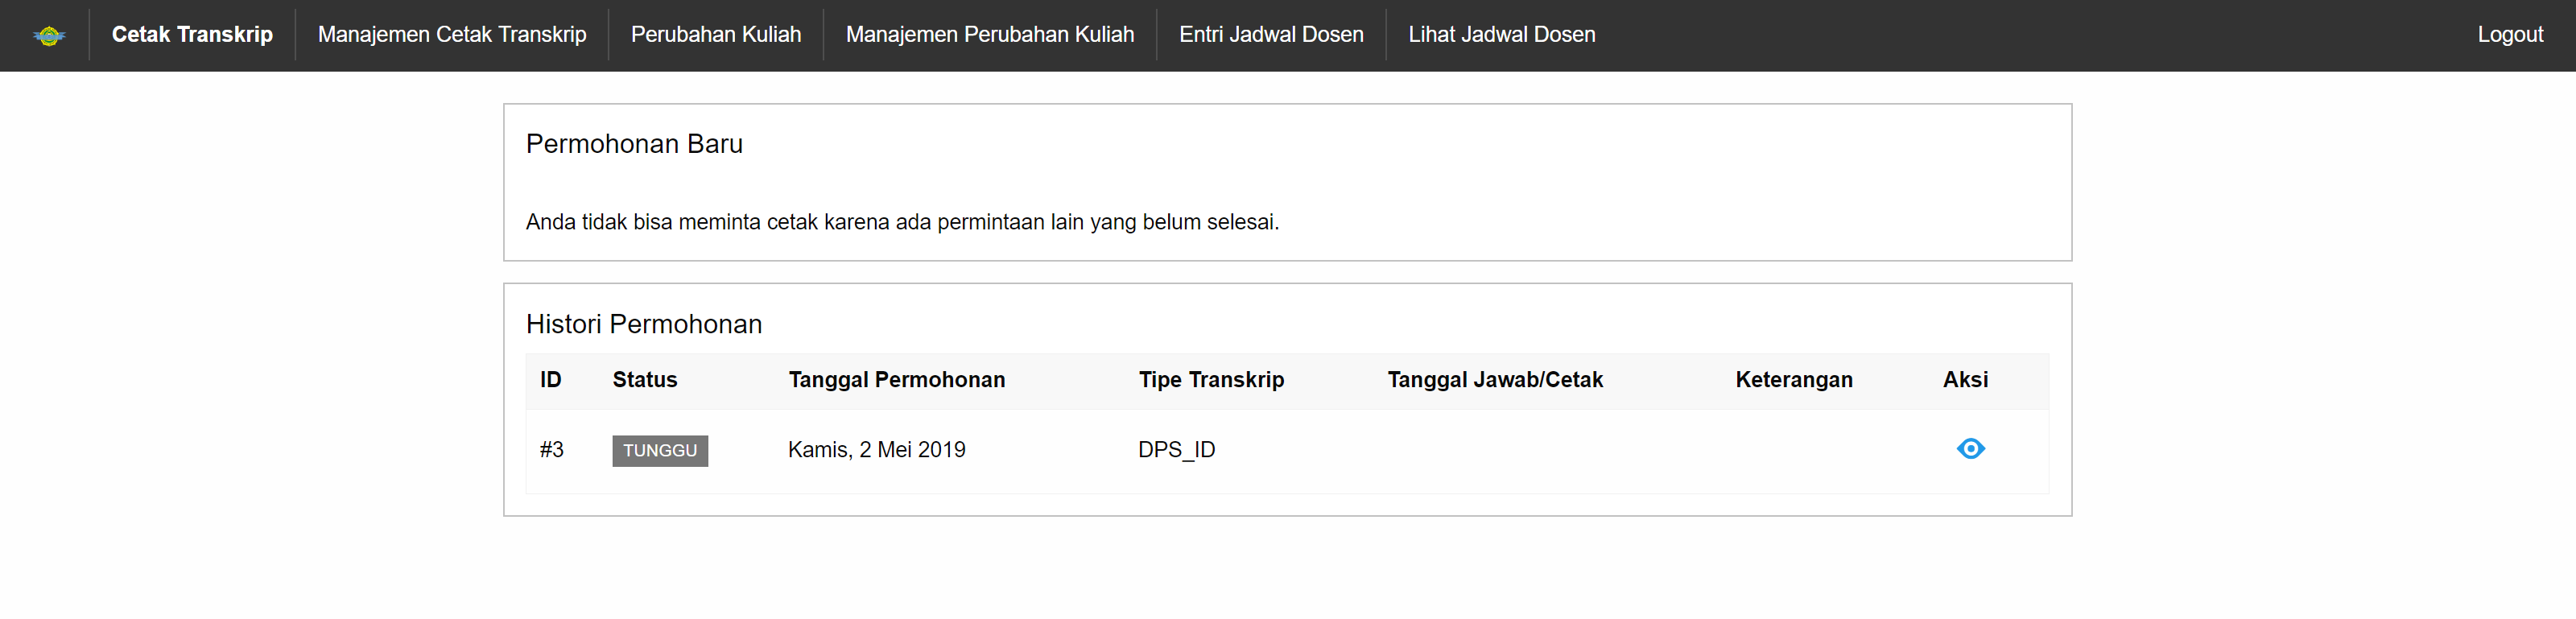
\includegraphics[scale=0.5]{Tampilan-Cetak-Transkrip.png}  
	\caption{Antarmuka Cetak Transkrip bagian 2} 
\end{figure}
Detail dari tabel permohonan baru :
\begin{itemize}
	\item \texttt{Yang memohon} : Berisi email UNPAR mahasiswa, otomatis terisi saat login melalui gmail.
	\item \texttt{NPM} : Berisi NPM mahasiswa yang ter-\textit{generate} secara otomatis.
	\item \texttt{Nama} : Nama mahasiswa yang tergenerate secara otomatis.
	\item \texttt{Tipe Transkrip} : Terdiri dari tiga pilihan yaitu DPS Bahasa Indonesia(Seluruh Semester), DPS Bahasa Inggris(Seluruh Semester), LHS (Semester Terakhir). Wajib diisi.
	\item Keperluan : Keterangan keperluan dibuat nya transkrip, wajib diisi mahasiswa.
\end{itemize}
Apabila ada form yang belum diisi maka akan terdapat \textit{warning} untuk \textit{field} yang kosong.
Berikut ini apabila mahasiswa menekan tombol aksi lihat 
\includegraphics[height=0.7\baselineskip]{tombol_eye.png} :
\begin{figure} [H]
	\centering  
	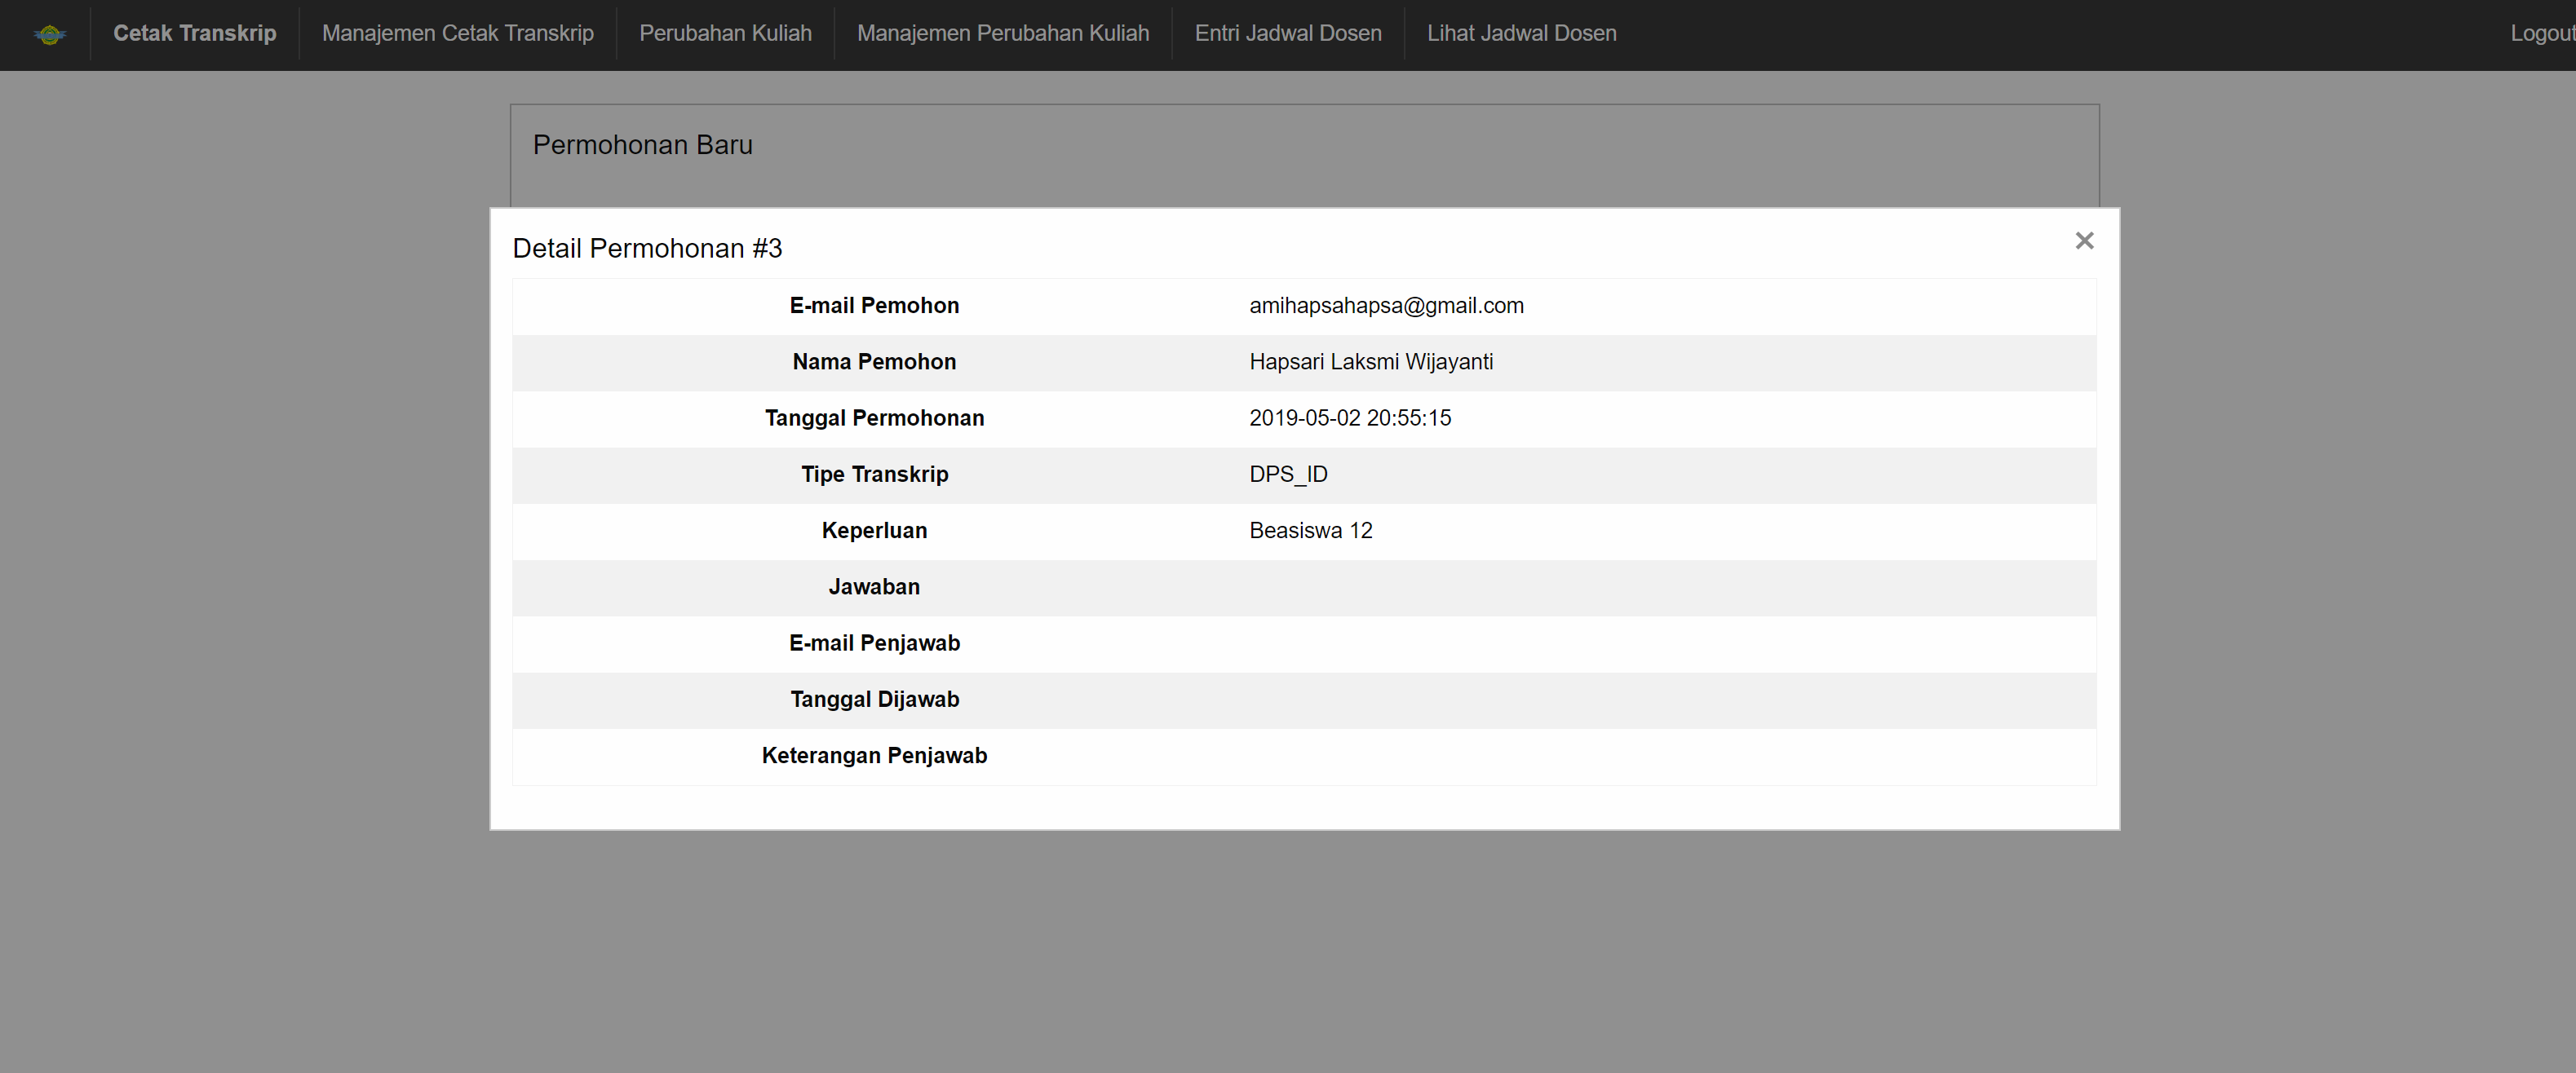
\includegraphics[scale=0.5]{Modal-Lihat-Cetak-Transkrip.png}  
	\caption{Modal Lihat Cetak Transkrip} 
\end{figure}
\noindent Disini aksi 'lihat' akan menampilkan sebuah modal yang berisi informasi detil permohonan, baik detil informasi dari mahasiswa maupun konfirmasi dari staf Tata Usaha.


\section{Antarmuka Manajemen Cetak Transkrip}
\begin{figure} [H]
	\centering  
	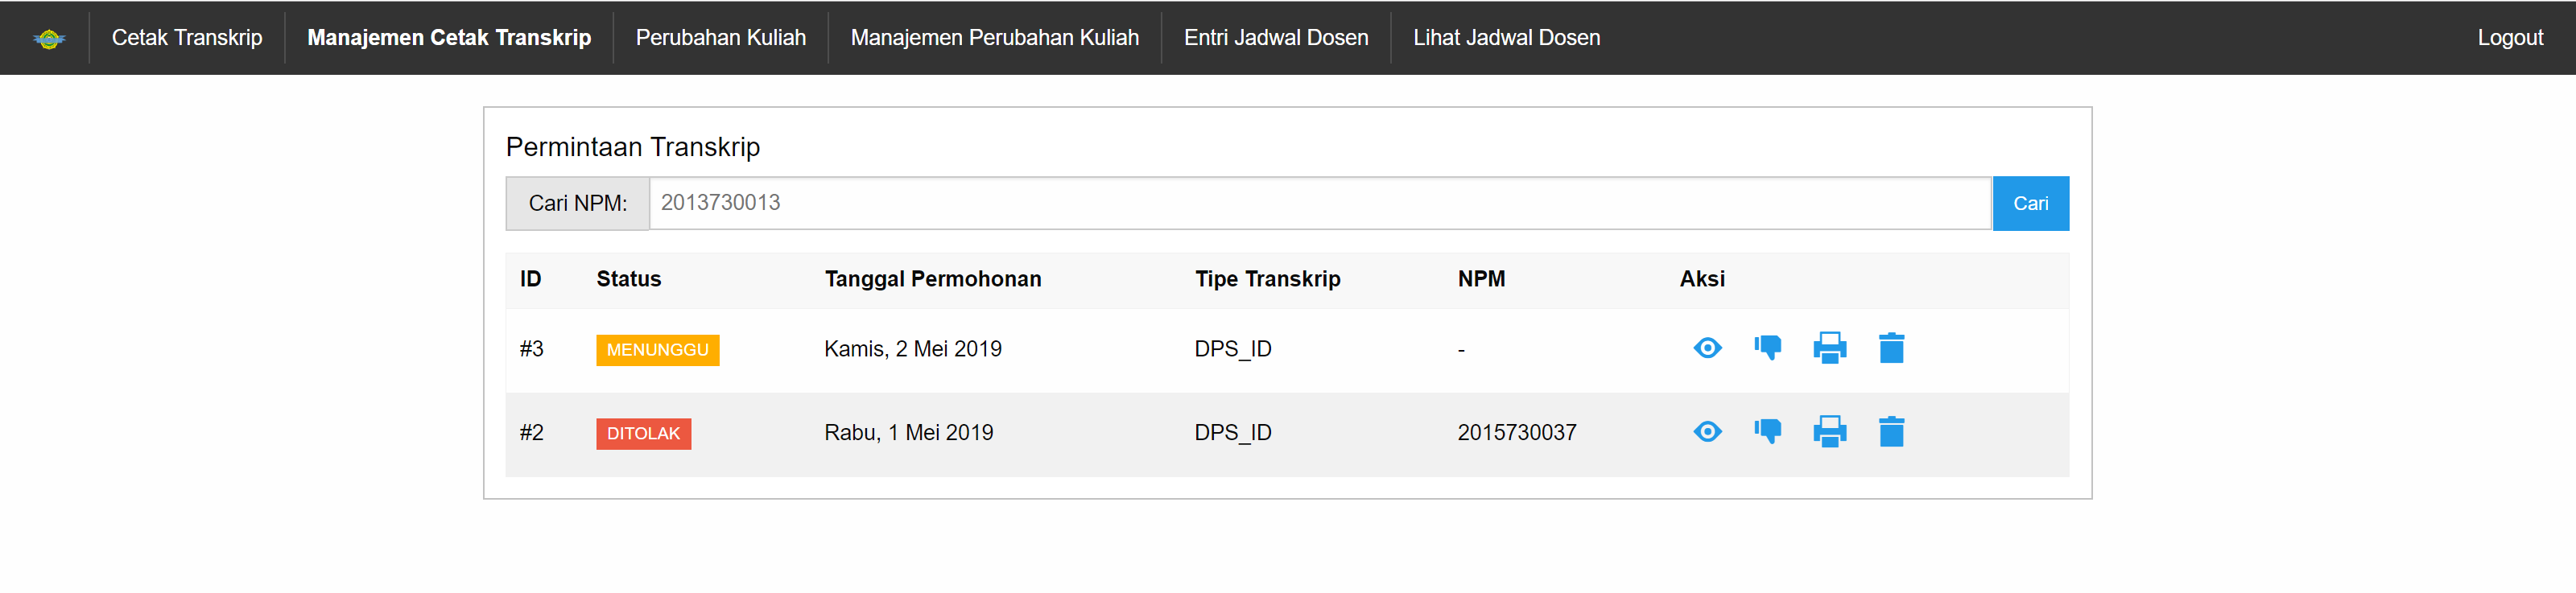
\includegraphics[scale=0.5]{Tampilan-Manajemen-Cetak-Transkrip.png}  
	\caption{Tampilan Manajemen Cetak Transkrip} 	
\end{figure}

Tampilan Manajemen Cetak Transkrip berisi sebuah tabel permintaan transkrip yang terdiri dari daftar permintaan transkrip dan form pencarian transkrip berdasarkan NPM.

\noindent Detail penjelasan untuk field 'Status' dan 'Aksi' :
\begin{itemize}
	\item[ ] \texttt{Status} : Output terdiri dari tiga jenis label yaitu 'MENUNGGU'(berwarna kuning), 'DITOLAK' (berwarna merah) dan 'TERCETAK'(berwarna hijau). 
	\item[ ] \texttt{Aksi} : Terdiri dari empat perintah yang akan menampilkan modal berisi informasi yang sesuai dengan perintah.
\end{itemize}

\begin{figure} [H]
	\centering  
	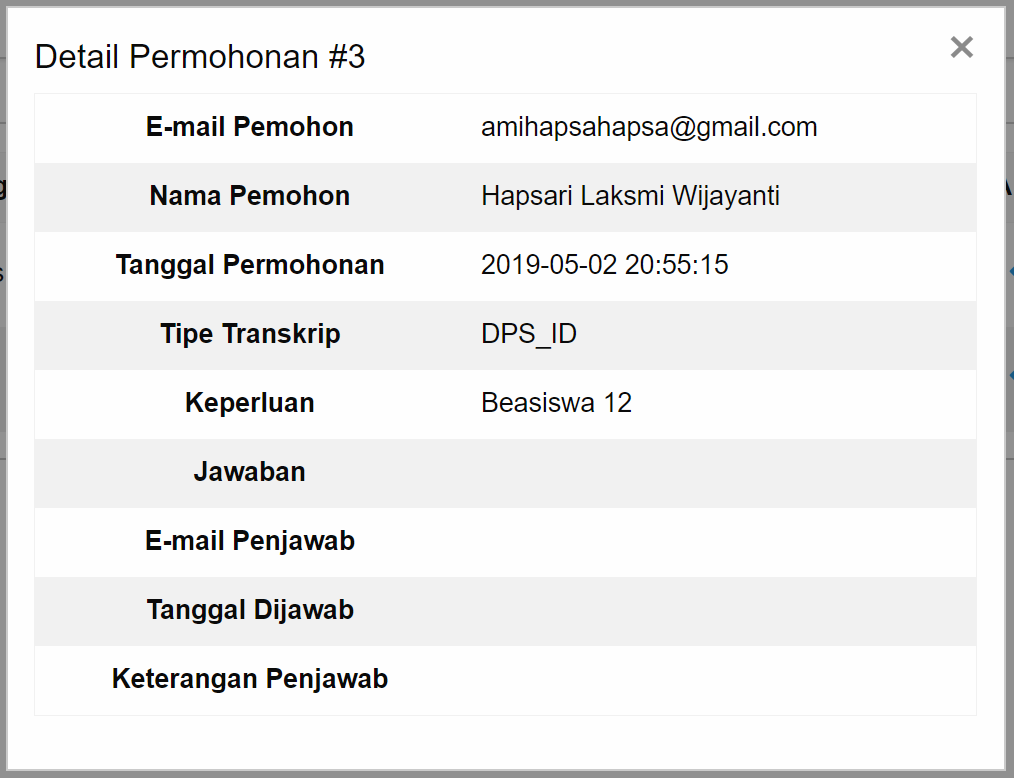
\includegraphics[scale=0.5]{Modal-Lihat-Manajemen-Cetak-Transkrip.png}  
	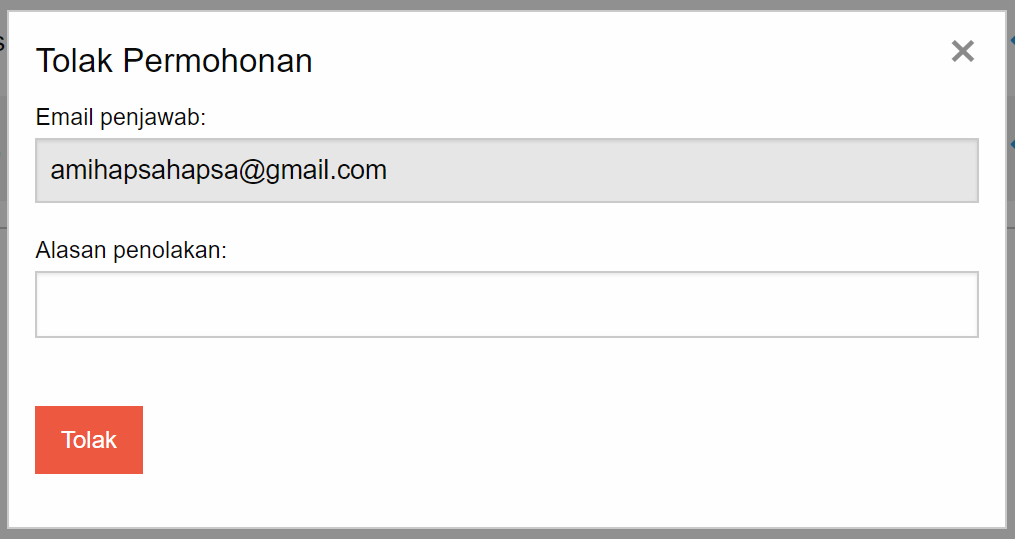
\includegraphics[scale=0.5]{Modal-Tolak-Manajemen-Cetak-Transkrip.png} 
	\caption{Tampilan Modal untuk aksi 'Lihat' dan 'Tolak'} 	
\end{figure}
\begin{figure} [H]
	\centering  
	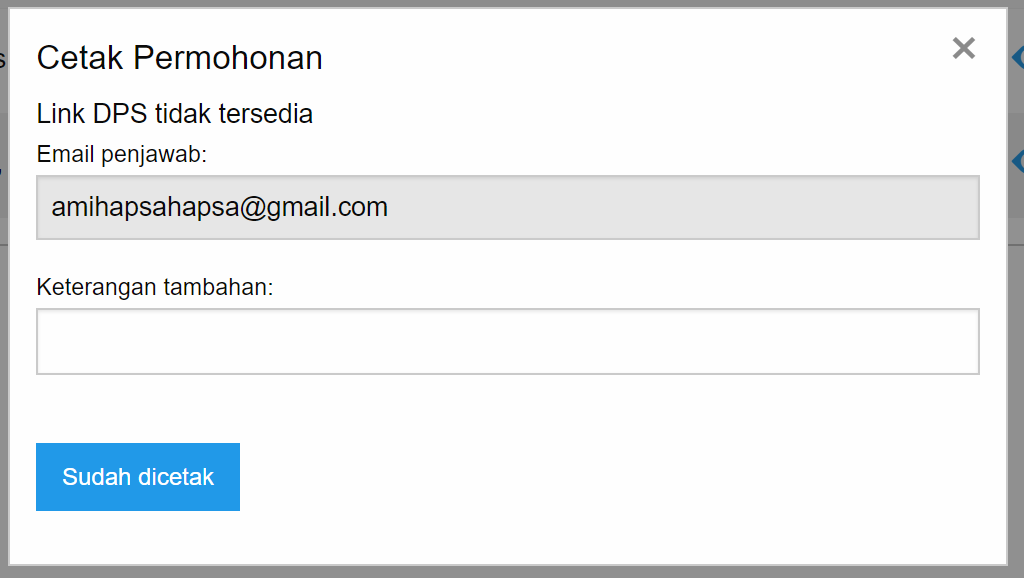
\includegraphics[scale=0.5]{Modal-Print-Manajemen-Cetak-Transkrip.png}  
	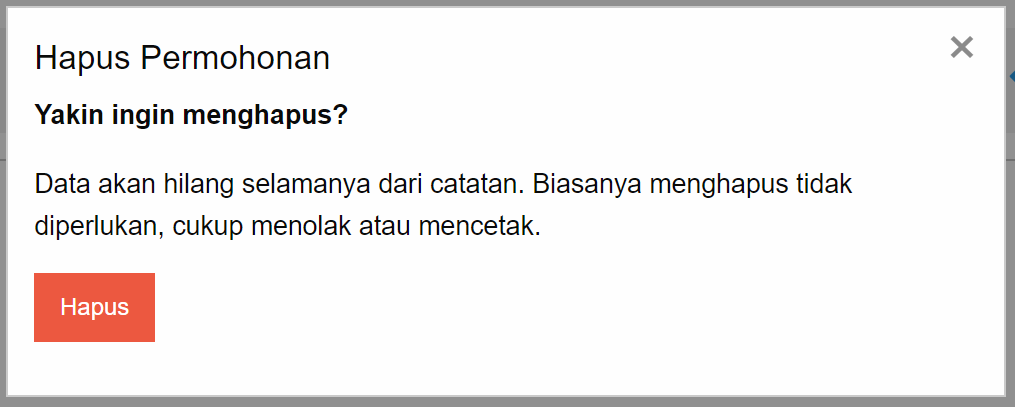
\includegraphics[scale=0.5]{Modal-Hapus-Manajemen-Cetak-Transkrip.png} 
	\caption{Tampilan Modal untuk aksi 'Print' dan 'Hapus'} 	
\end{figure}

 
\section{Antarmuka Perubahan Kuliah}
\begin{figure} [H]
	\centering  
	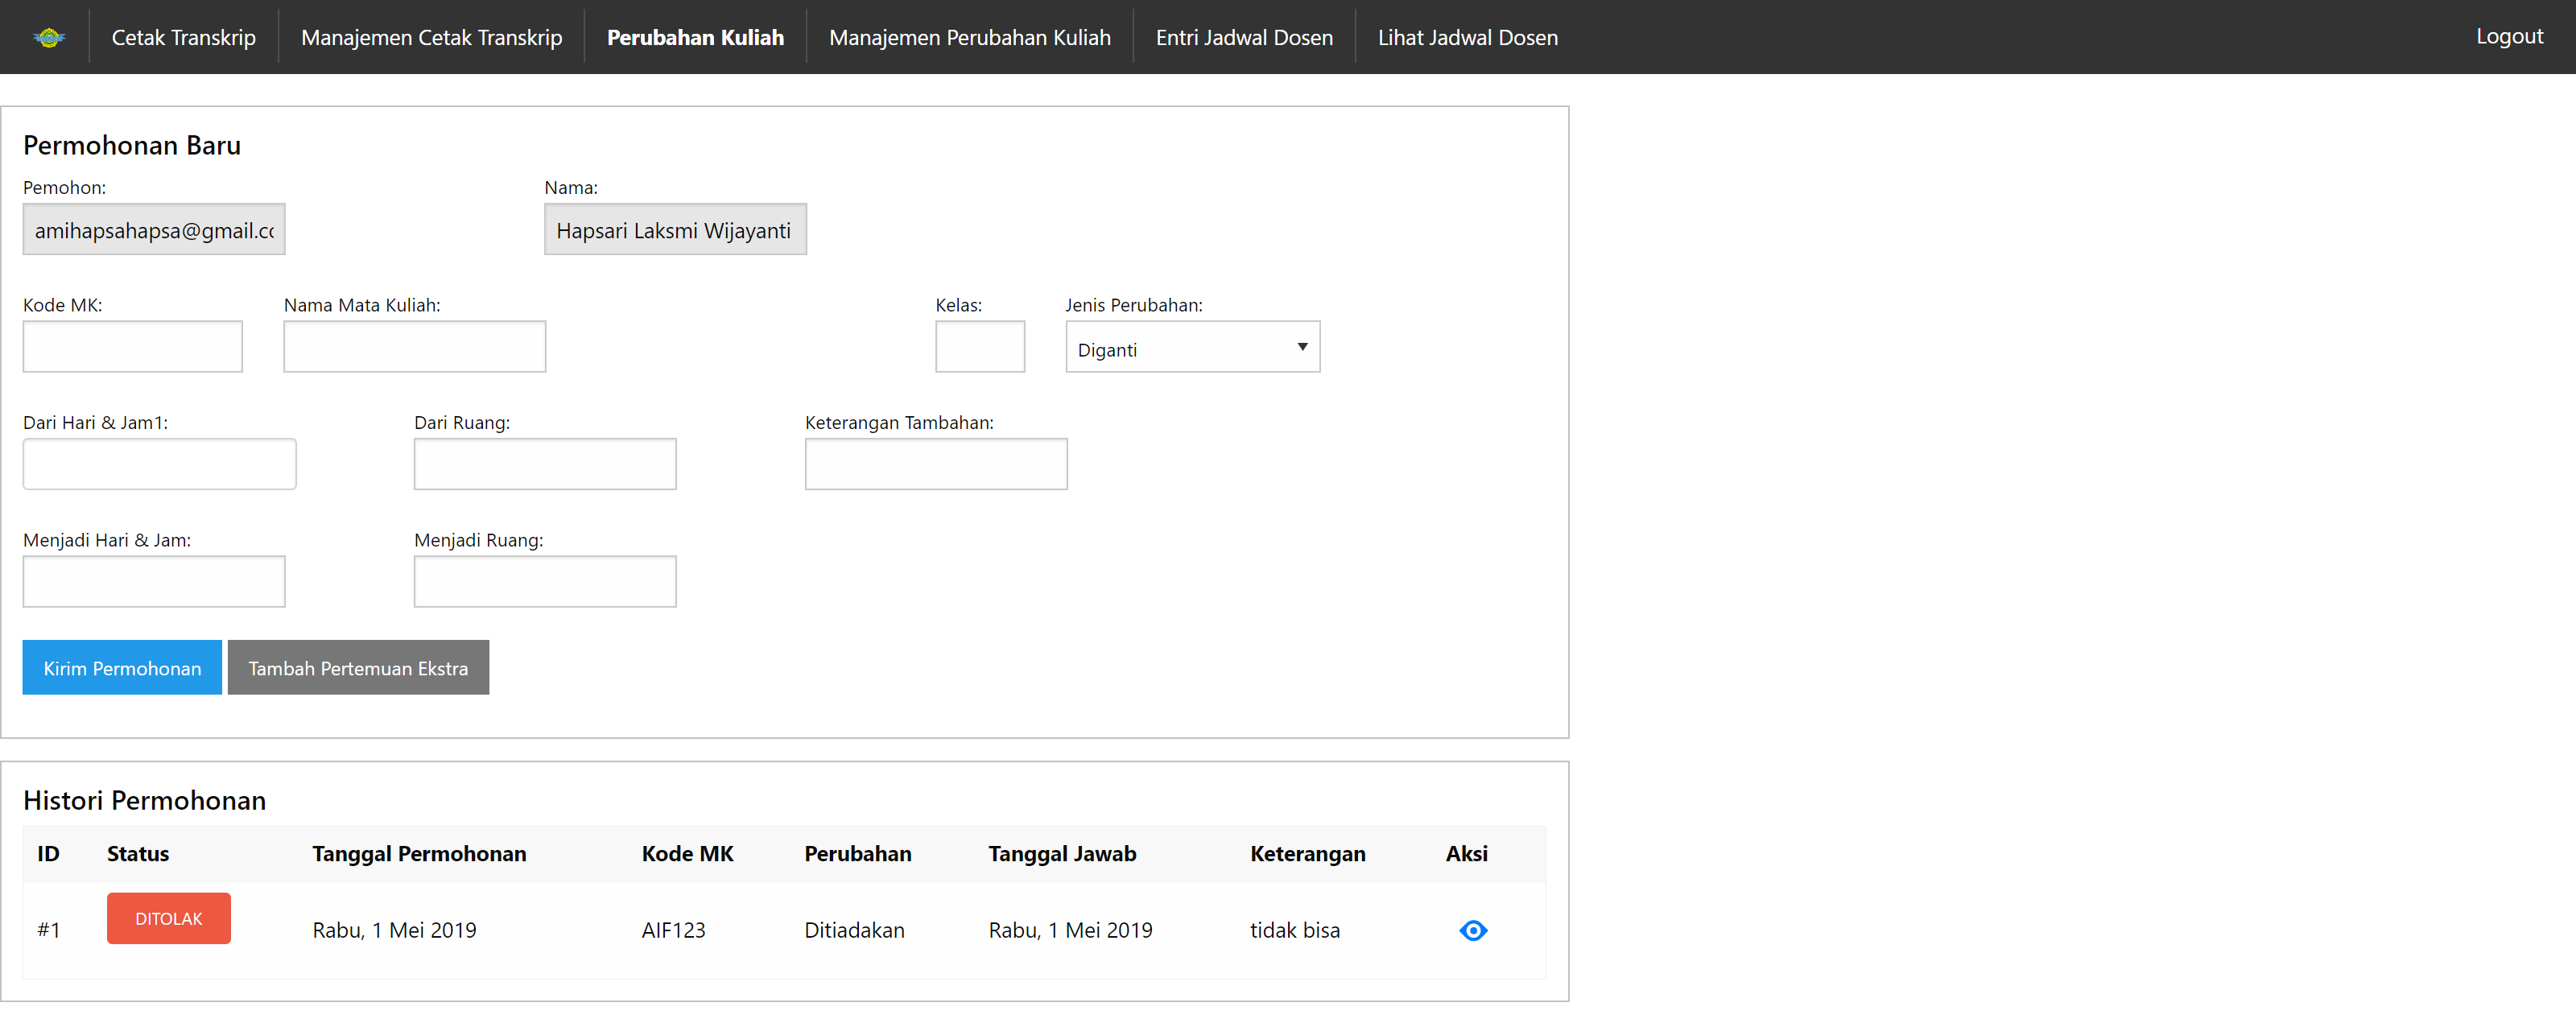
\includegraphics[scale=0.5]{Tampilan-Perubahan-Kuliah.png}  
	\caption{Tampilan Perubahan Kuliah} 
\end{figure}
Modul Perubahan Kuliah terdiri dari dua tabel yaitu :

\subsection{Permohonan Baru}

\begin{tabular}{ |p{4cm}|p{2cm}|p{10cm}|  }
	\hline
	Nama Kolom & Pilihan & Keterangan\\
	\hline
	\texttt{Pemohon} &  &Field terisi secara otomatis, user tidak bisa mengisi field atau \textit{disabled} \\
	\hline
	\texttt{Nama} &    & Field terisi secara otomatis, user tidak bisa mengisi field atau \textit{disabled}\\
	\hline
	\texttt{Kode MK } & & Field bertipe text \\
	\hline
	\texttt{Nama Mata Kuliah}    & & Field bertipe text \\
	\hline
	\texttt{Kelas} &  & Field bertipe text \\
	\hline
	\texttt{Jenis Perubahan} & Diganti &  Field 'Dari Hari dan Jam' dan 'Dari Ruang' disabled  \\
	 & Tambahkan &    Field 'Dari Hari dan Jam' dan 'Dari Ruang' dapat ditambahkan lebih dari satu kolom\\	 
	 & Ditiadakan &  Field 'Menjadi Hari dan Jam' dan 'Menjadi Ruangan' disabled   \\
	\hline
	\texttt{Dari Hari dan Jam} &  & Menggunakan plugin \textit{calendar} \\
	\hline
	\texttt{Dari Ruang} &  & Field bertipe text \\
	\hline
	\texttt{Keterangan Tambahan} &  & Field bertipe text \\
	\hline
	\texttt{Menjadi Hari dan Jam} &  & Menggunakan plugin \textit{calendar} \\
	\hline
	\texttt{Menjadi Ruangan} &  & Field bertipe text \\
	\hline
\end{tabular}

\subsection{Histori Pemohonan}
\begin{tabular}{ |p{4cm}|p{2cm}|p{10cm}|  }
	\hline
	Nama Kolom & Pilihan & Keterangan\\
	\hline
	\texttt{Status} & dikonfirmasi & Apabila staf TU menyetujui permohonanan\\
	\hline
	&  ditolak  & Apabila staf TU menolak permohonanan\\
	\hline
	& ditunggu &  Apabila staf TU belum konfirmasi permohonan \\
	\hline
	\texttt{Tanggal Permohonan}    & & Data bertipe tanggal \\
	\hline
	\texttt{Kode MK} &  & Field bertipe text \\
	\hline
	\texttt{Perubahan} &  &  Konfirmasi staf TU : Diganti, Ditambahkan, Ditiadakan \\
	\hline
	\texttt{Tanggal Jawab} &  & Data bertipe tanggal \\
	\hline
	\texttt{Keterangan} &  & Field bertipe text \\
	\hline
	\texttt{Aksi} &  & Terdapat tombol aksi 'Lihat' \\
	\hline
\end{tabular}
Ketika user menekan tombol aksi 'lihat', maka modal berisi informasi data permohonan yang sesuai dengan ID 
\begin{figure} [H]
	\centering  
	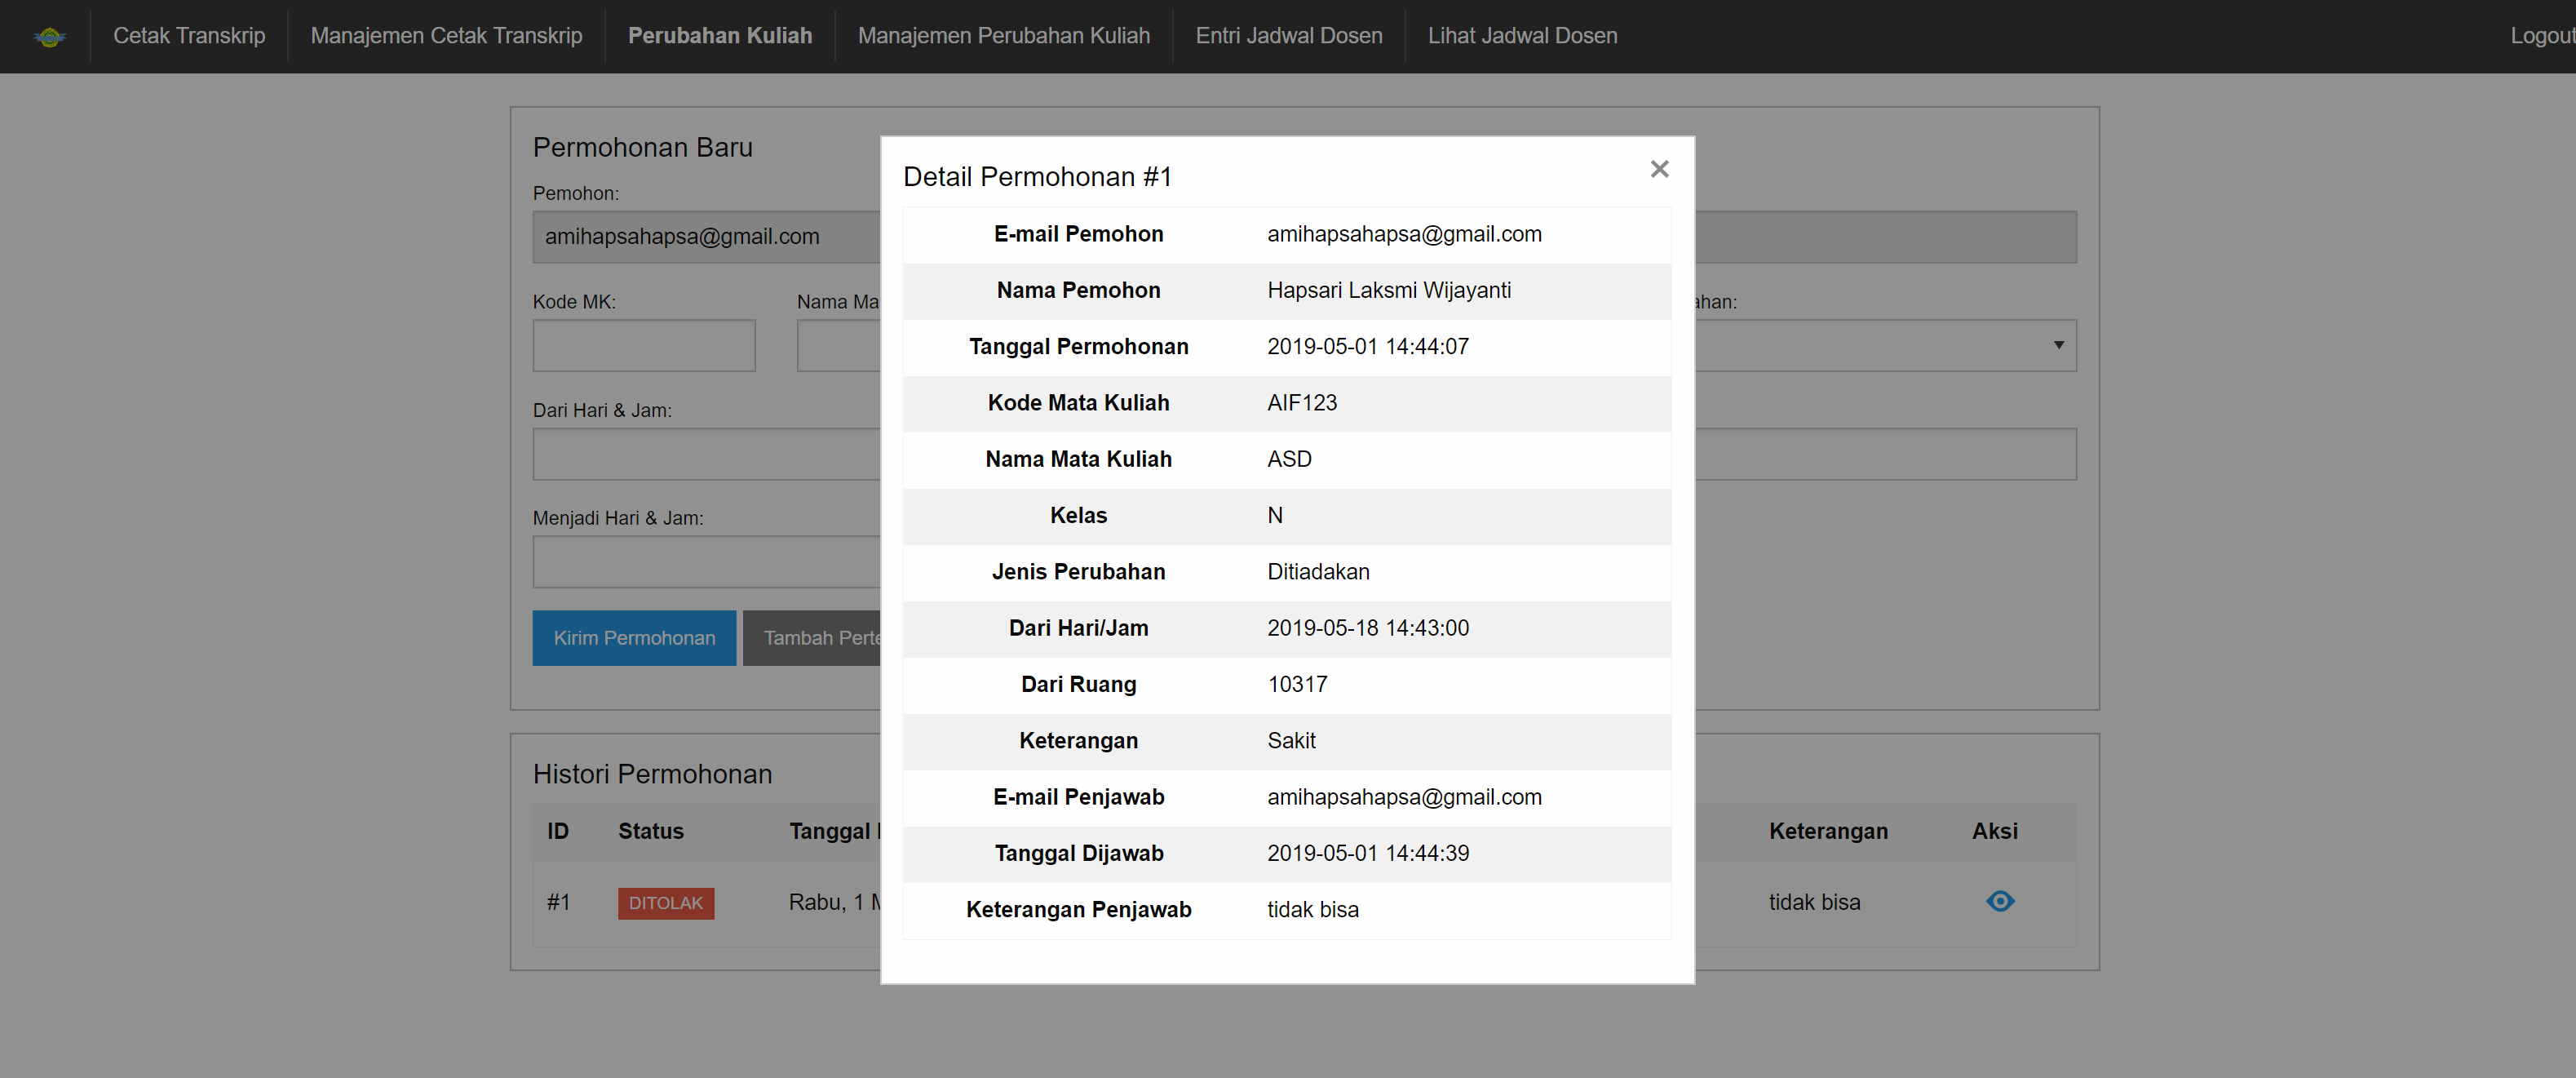
\includegraphics[scale=0.5]{Modal-Lihat-Perubahan-Kuliah.png}  
	\caption{Modal Lihat Perubahan Kuliah} 
\end{figure}


\section{Antarmuka Manajemen Perubahan Kuliah}
\begin{figure} [H]
	\centering  
	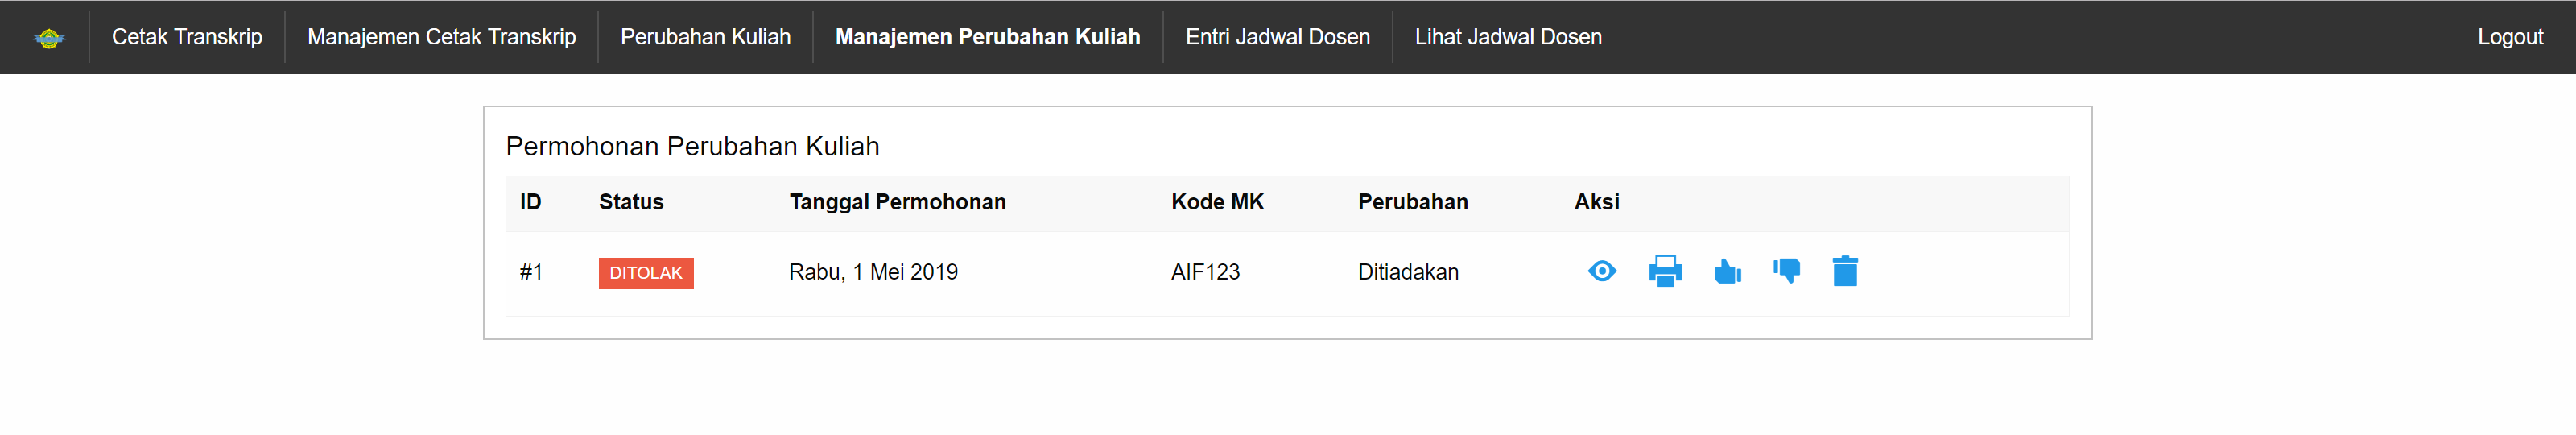
\includegraphics[scale=0.5]{Tampilan-Manajemen-Perubahan-Kuliah.png}  
	\caption{Tampilan Manajemen Perubahan Kuliah} 
\end{figure}
Tabel Pemohonan Kuliah memiliki detail yang sama dengan tabel histori permohonan, namun aksi yang dilakukan terdiri dari lima perintah:
\begin{figure} [H]
	\centering  
	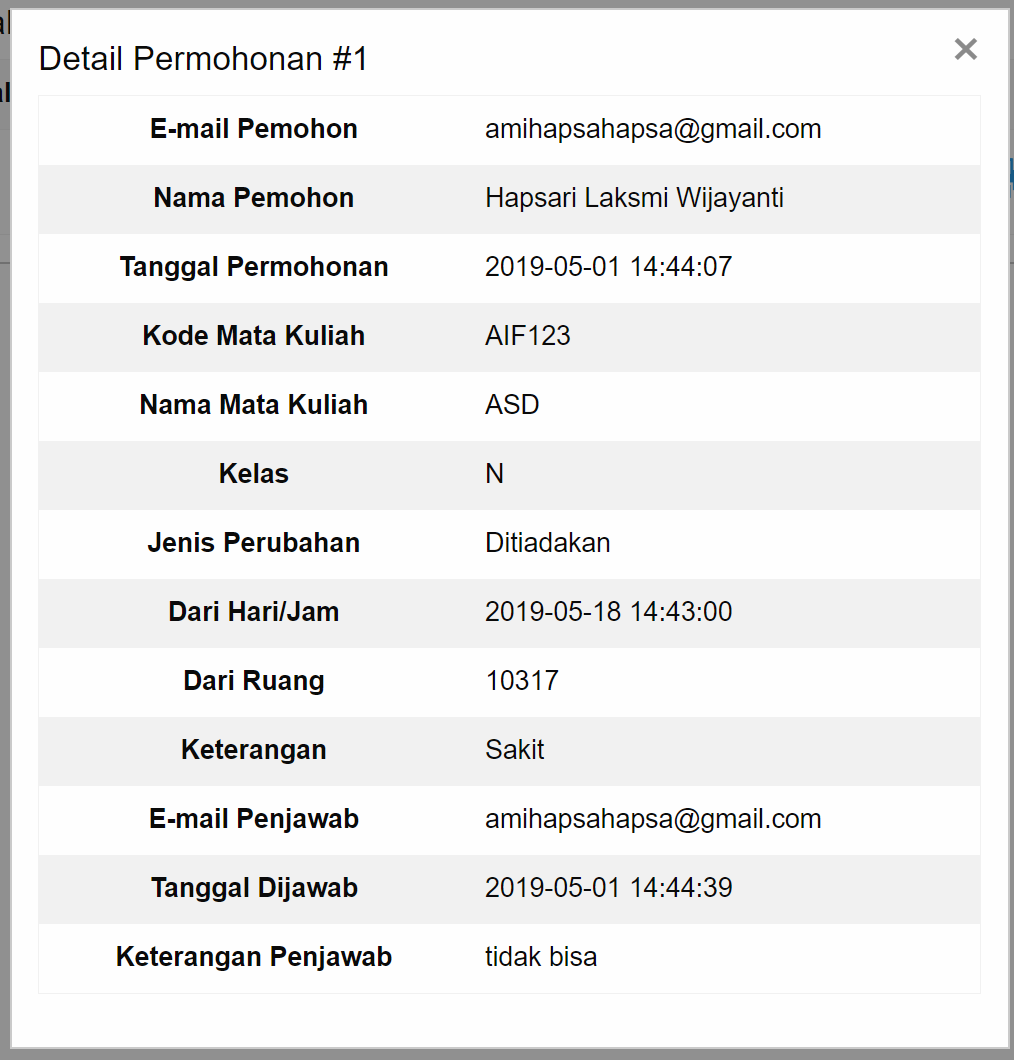
\includegraphics[scale=0.3]{Modal-Lihat-Manajemen-Perubahan-Kuliah.png}  
	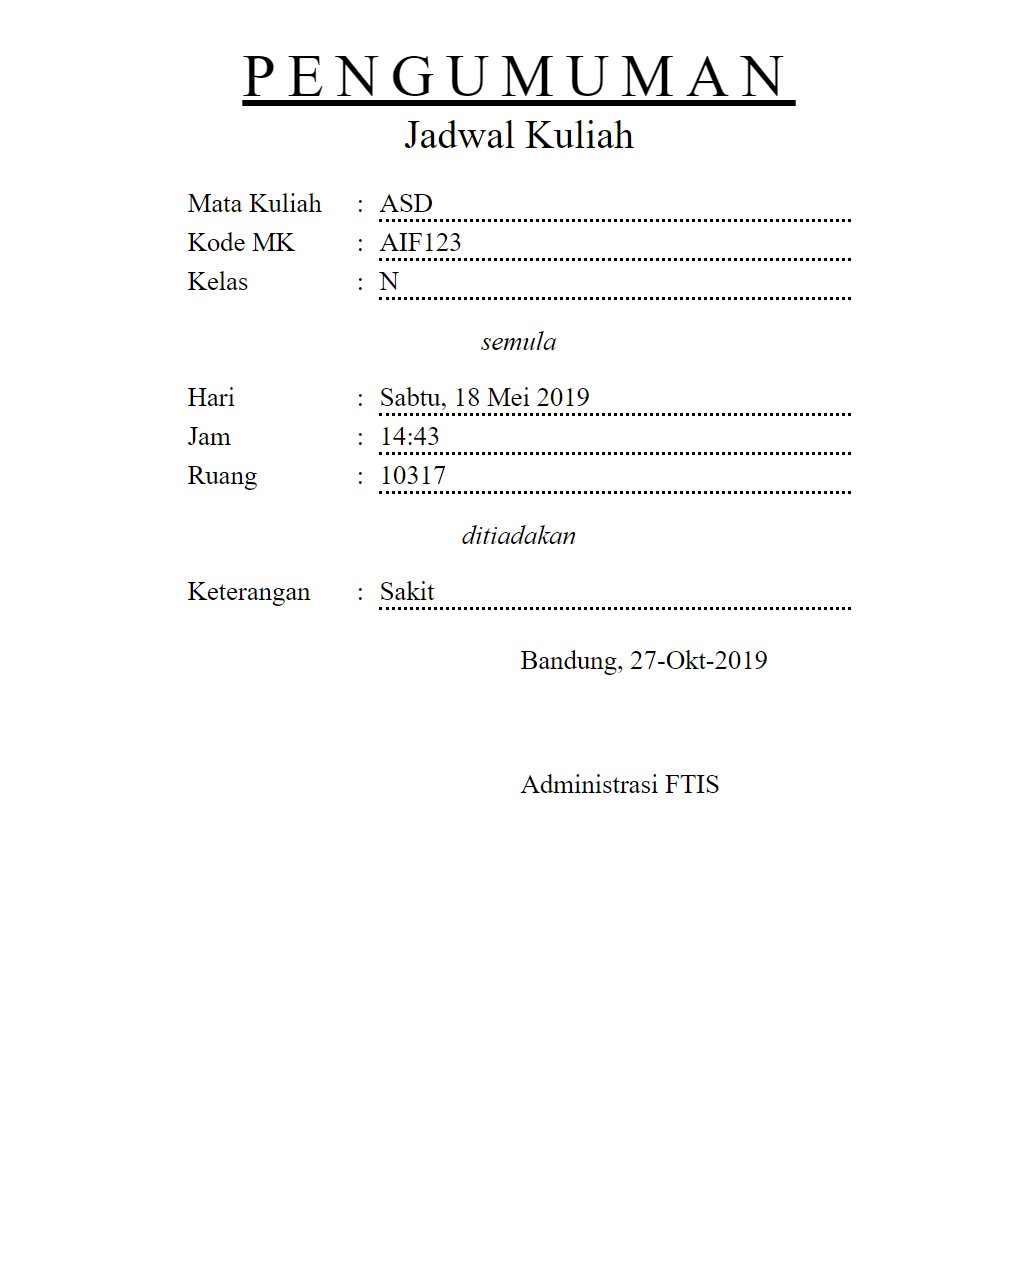
\includegraphics[scale=0.3]{Modal-Print-Manajemen-Perubahan-Kuliah.png} 
	\caption{Modal aksi Lihat dan Print Manajemen Perubahan Kuliah} 
\end{figure}
\begin{figure} [H]
	\centering  
	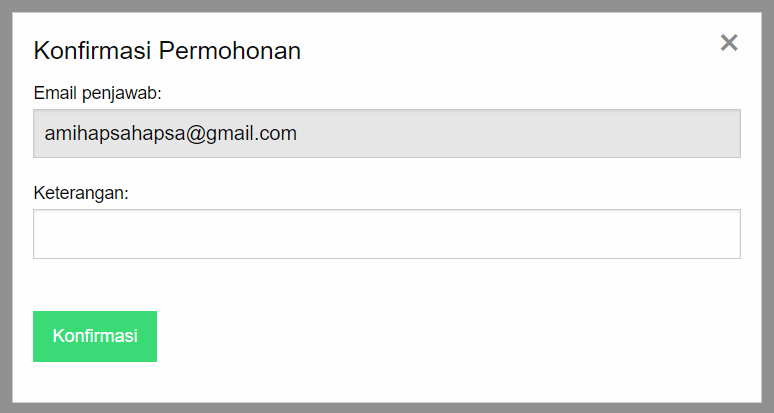
\includegraphics[scale=0.3]{Modal-Setuju-Manajemen-Perubahan-Kuliah.png}
	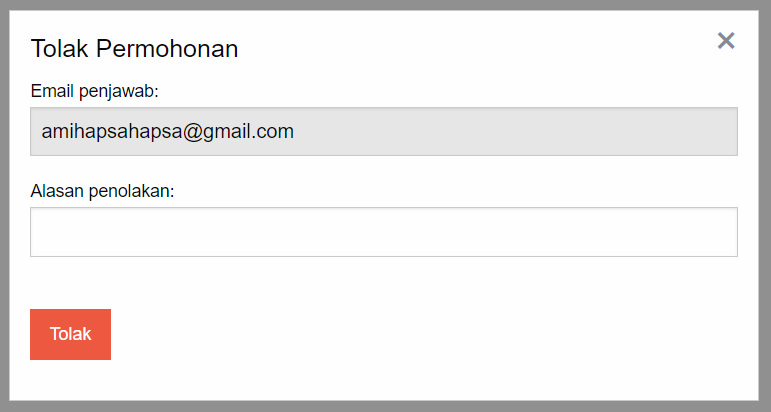
\includegraphics[scale=0.3]{Modal-Tolak-Manajemen-Perubahan-Kuliah.png}    
	\caption{Modal aksi Setuju dan Tolak Manajemen Perubahan Kuliah} 
\end{figure}
\begin{figure} [H]
	\centering  
	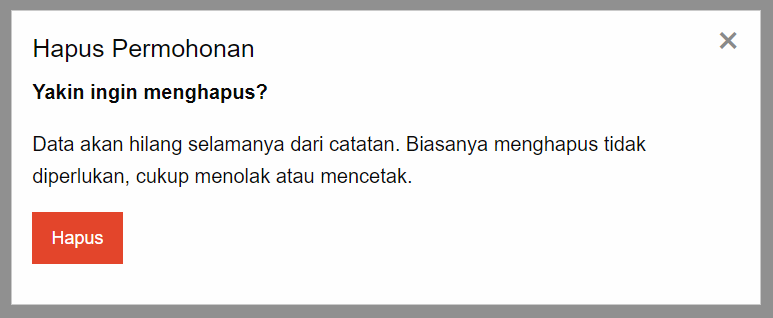
\includegraphics[scale=0.3]{Modal-Hapus-Manajemen-Perubahan-Kuliah.png}  
	\caption{Modal Hapus Manajemen Perubahan Kuliah} 
\end{figure}

\section{Antarmuka Entri Jadwal Dosen}
\begin{figure} [H]
	\centering  
	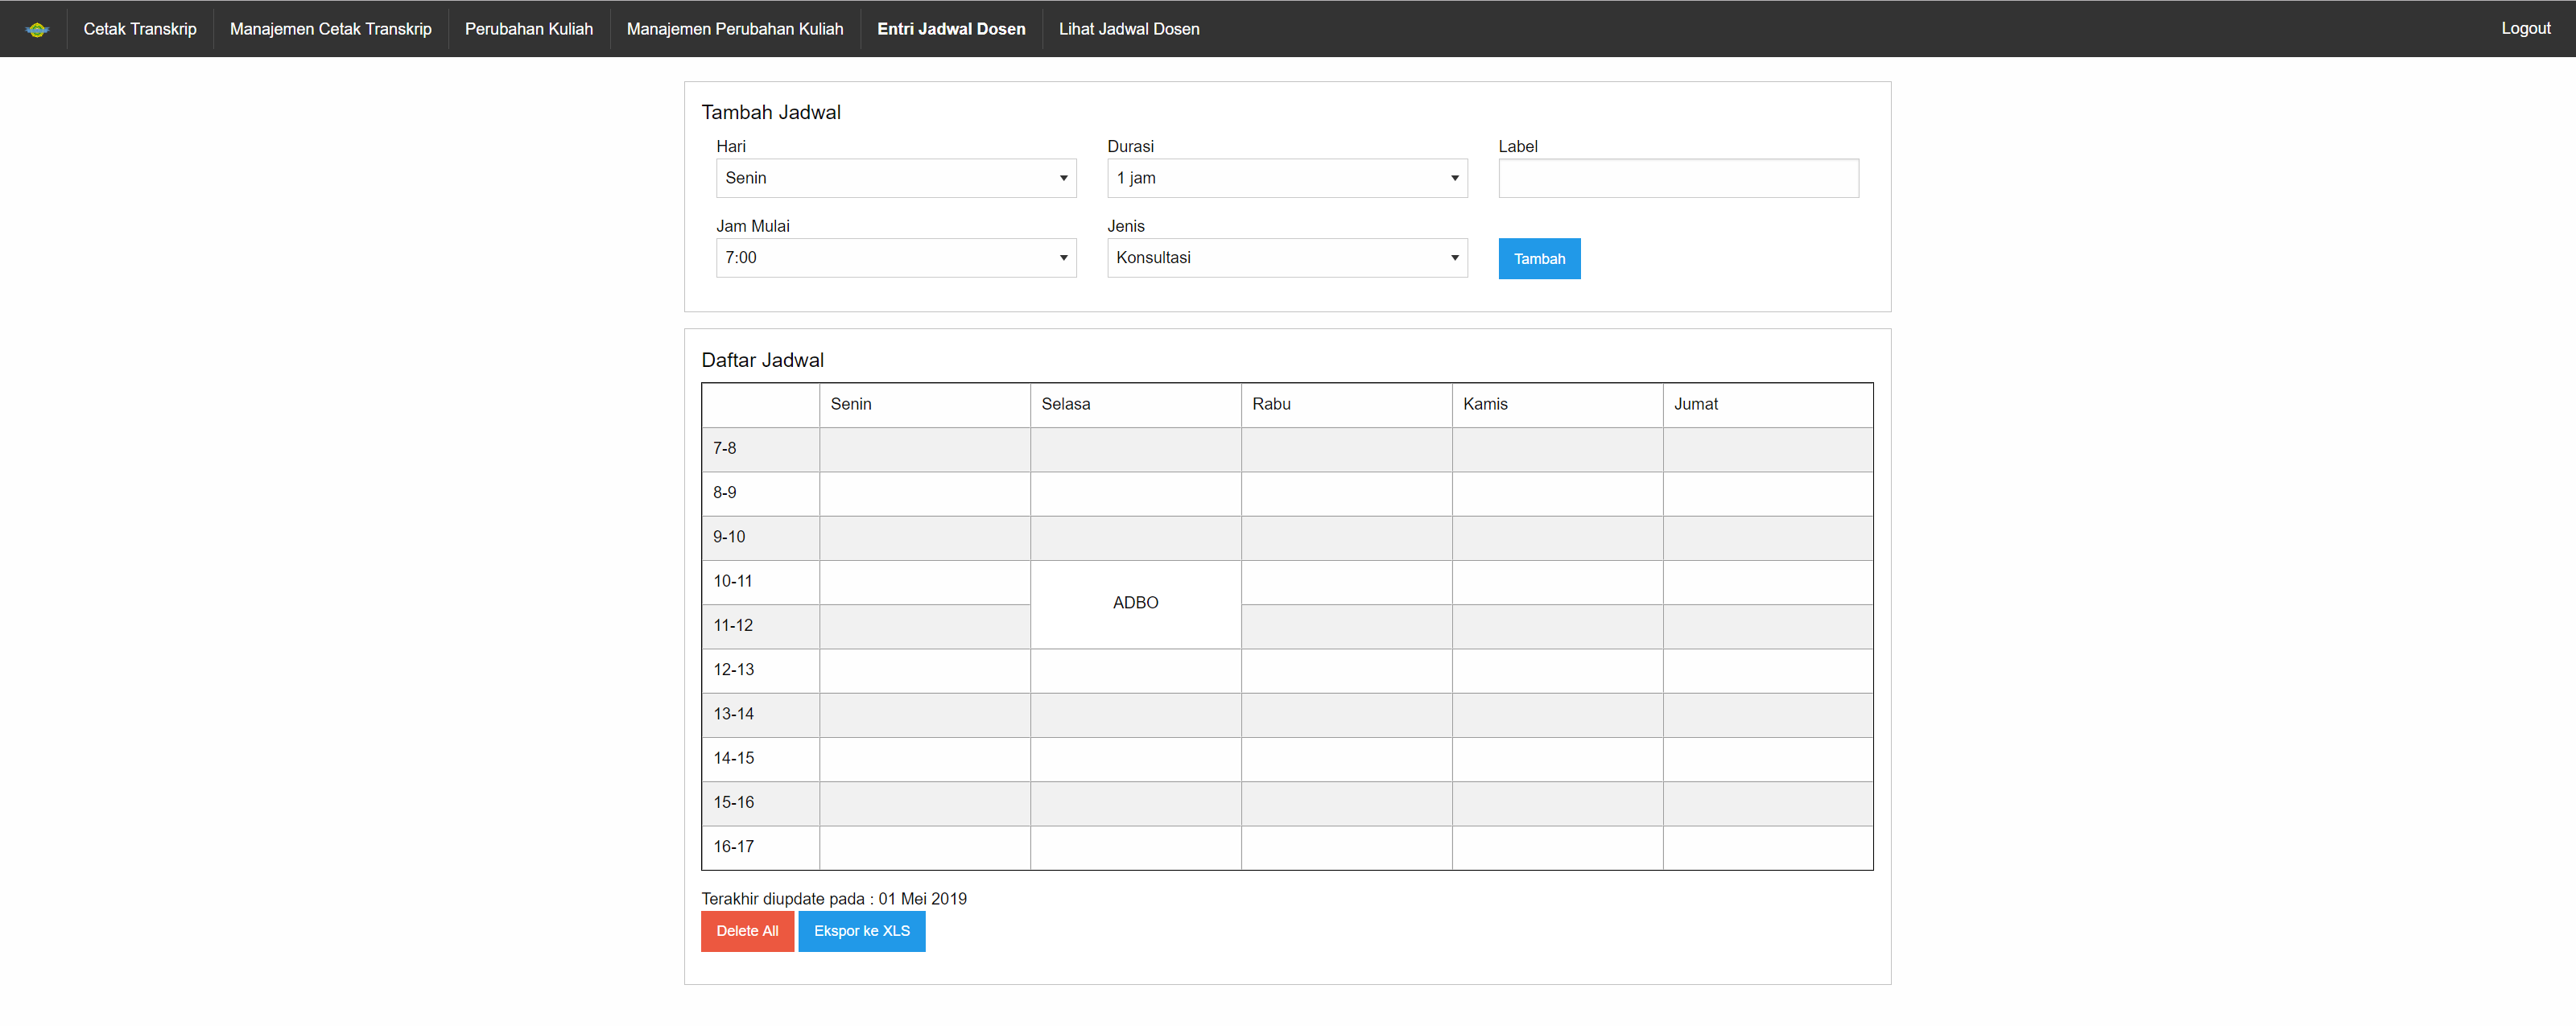
\includegraphics[scale=0.5]{Tampilan-Entri-Jadwal-Dosen.png}  
	\caption{Modal Print Manajemen Perubahan Kuliah} 
\end{figure}
Detail mengenai tabel Tambah Jadwal :
\begin{itemize}
	\item \texttt{Hari} : Terdiri dari nama hari dari senin sampai jumat.
	\item \texttt{Durasi} : Terdiri dari rentang jam kelas berlangsung dari 1 jam hingga 9 jam.
	\item \texttt{Label} : Field bertipe text.
	\item \texttt{Jam Mulai} : Terdiri dari jam dari rentang 07:00 sampai 16:00.
	\item \texttt{Jenis} : Terdiri dari tiga macam pilihan 
	\begin{enumerate}
		\item Konsultasi : Memiliki background berwarna hijau.
		\item Terjadwal : Memiliki background berwarna biru.
		\item Kelas : Memiliki background putih.
	\end{enumerate}
\end{itemize}

Tabel Daftar jadwal akan \textit{retrieve} data jadwal dari dosen yang dibuat. Terdiri dari rentang waktu dan hari. Jadwal yang terlihat pada tabel ini bisa diedit dan dihapus.
Dibagian bawah tabel akan terlihat tanggal jadwal tersebut di update dan memiliki dua tombol :
\begin{itemize}
	\item \texttt{Delete All} : Menghapus semua jadwal yang sudah dibuat.
	\item \texttt{Export ke XLS} : Secara otomatis akan membuat file excel dan mendownload di device secara lokal.
\end{itemize}

\section{Antarmuka Lihat Jadwal Dosen}
\begin{figure} [H]
	\centering  
	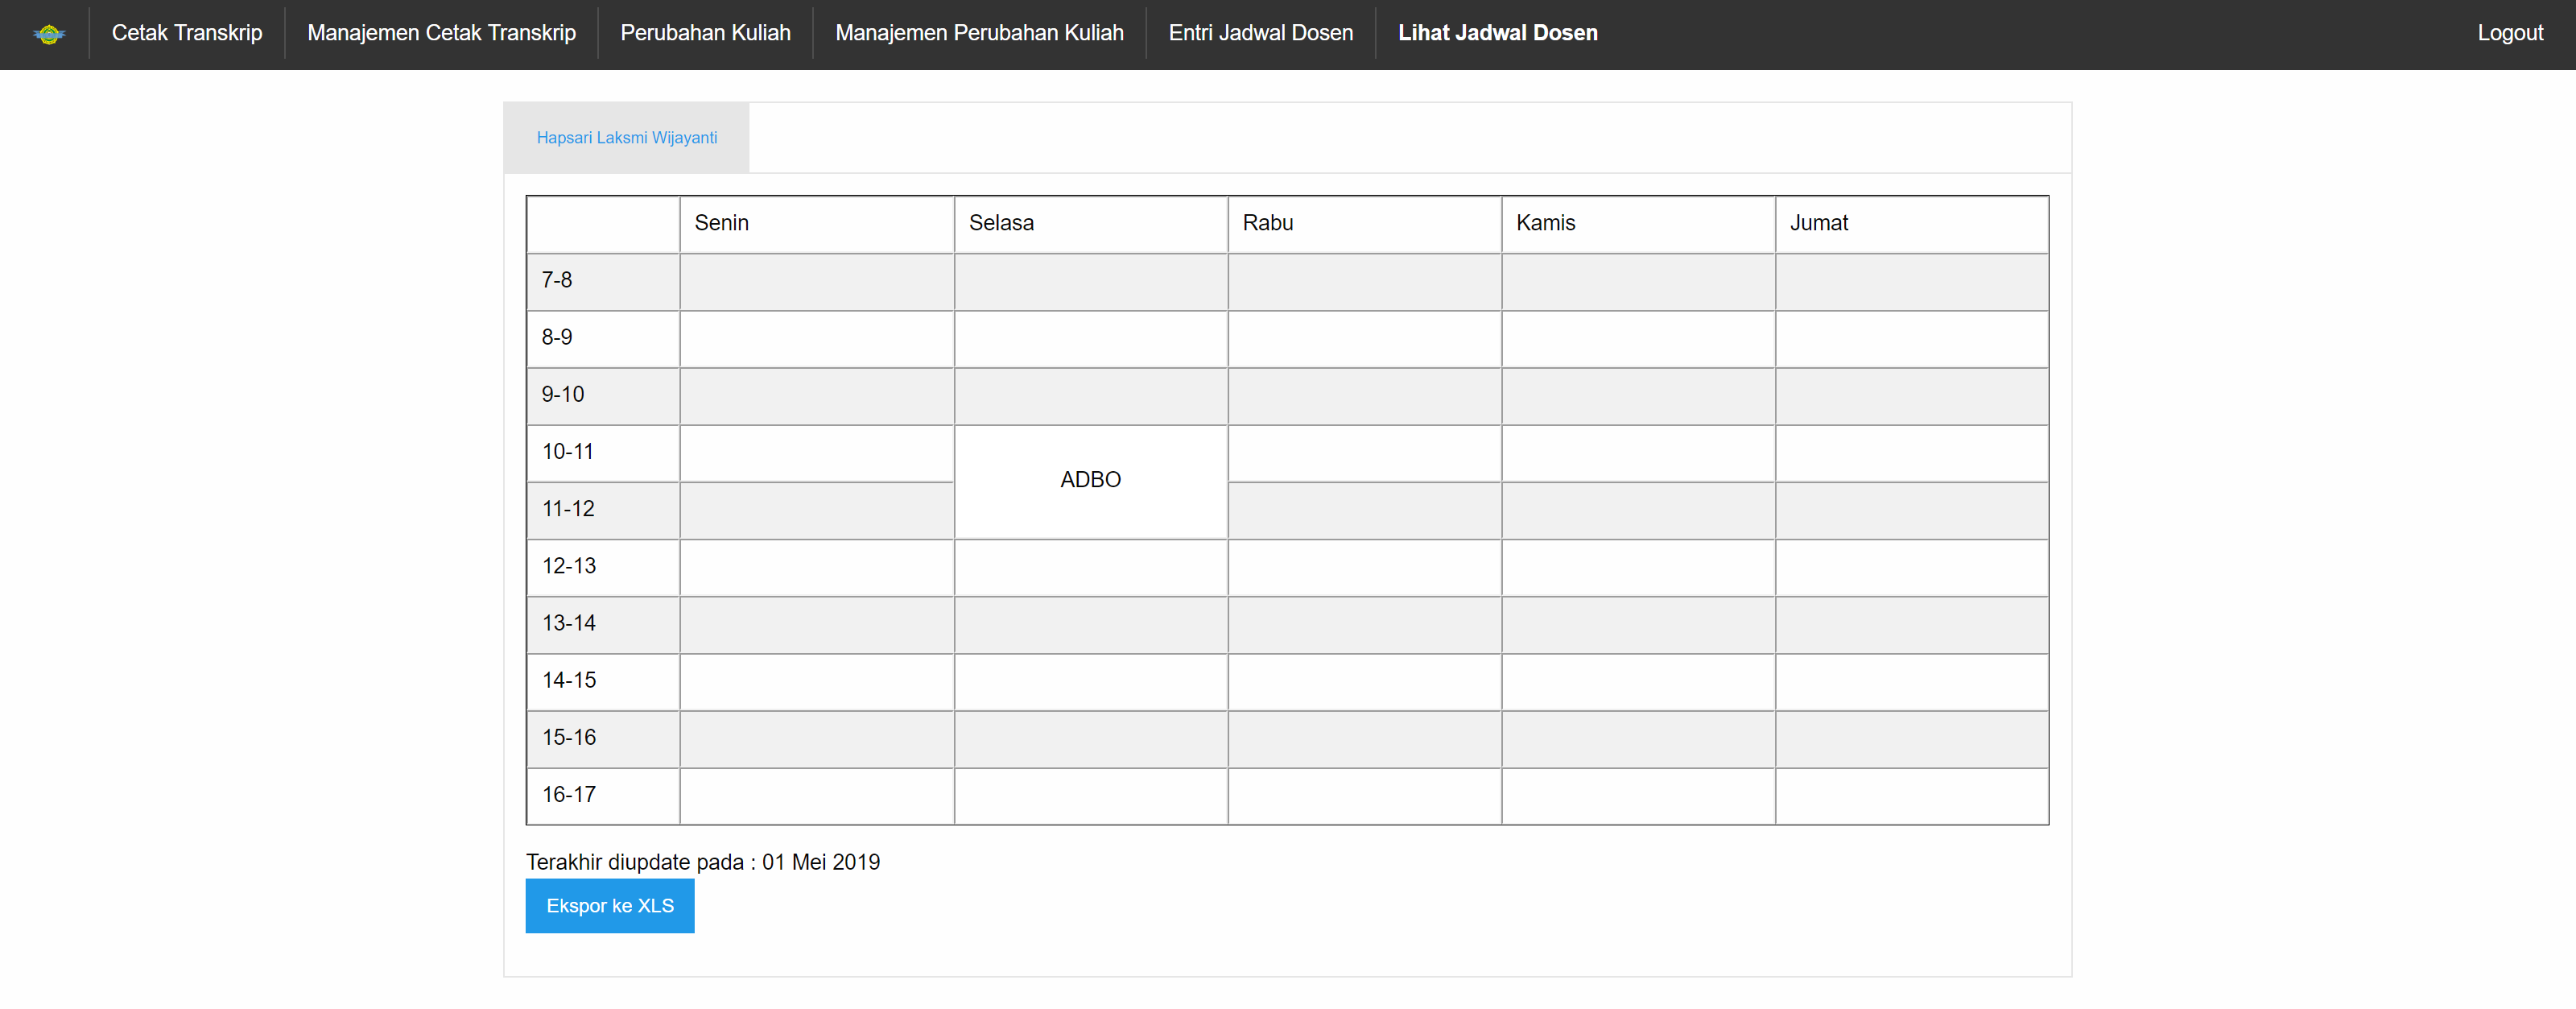
\includegraphics[scale=0.5]{Tampilan-Lihat-Jadwal-Dosen.png}  
	\caption{Struktur File Zurb Foundation} 	
\end{figure}
Tabel Jadwal Dosen akan \textit{retrieve} data jadwal dari setiap dosen yang dibuat. Seluruh mahasiswa dapat mengakses halaman ini. Terdiri dari rentang waktu dan hari. 
Lalu akan terlihat tanggal kapan terakhir jadwal bisa.